\section{Correctness}

{\bf Isolating \phinode using copies}
In most cases, edge splitting can be avoided by treating symmetrically \phiuses and \phidef: instead of just inserting copies on the incoming control flow edges of the \phinode (one for each use operand), a copy is also inserted on the outgoing edge (one for its defining operand). This has the effect of isolating the value associated to the \phinode thus avoiding (as discussed further) SSA destruction issues such as the well known lost-copy problem.
The process of \phinode isolation is illustrated by Figure~\ref{fig:phi_isolation}.
The corresponding pseudo-code is given in Algorithm~\ref{alg:alternative_ssa_destruction:sreedhar}. If, because of different \phifuns, several copies are introduced at the
same place, they should be viewed as parallel copies. For that reason, an empty parallel copy is inserted both at the beginning (i.e., right after \phifuns, if any) and at the end of each basic-block (i.e., just before the branching operation, if any).  
Note that, as far as correctness is concerned, copies
can be sequentialized in any order, as they concern different
variables. 

\begin{figure}[h]
\subfloat[Initial code]{
  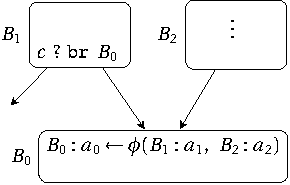
\includegraphics[scale=0.7]{phi_isolation_a.pdf}
}\hfill
\subfloat[After isolating the \phifun]{
  \hspace{2em}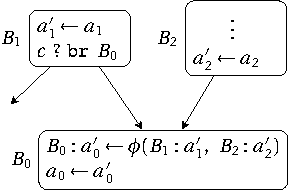
\includegraphics[scale=0.7]{phi_isolation_b.pdf}
}
\caption{Isolation of a \phinode\label{fig:phi_isolation}}
\end{figure}


When incoming edges are not split, inserting a copy not only for each argument of the \phifun, but also for its result is important: without the copy $a'_0\gets a_0$, the \phifun defines
directly~$a_0$ whose live range can be long enough to intersect the live range
of some $a'_i$, $i>0$, if $a_0$ is live out of the block~$B_i$ where~$a'_i$ is
defined. Two cases are possible: either $a_0$ is used in a successor of $B_i
\neq B_0$, in which case the edge from~$B_i$ to~$B_0$ is \emph{critical} (as in
the ``lost copy problem''), or $a_0$ is used in $B_0$ as a $\phi$-function
argument (as in the ``swap problem''). In this latter case, if parallel copies
are used, $a_0$ is dead before~$a'_i$ is defined but, if copies are
sequentialized blindly, the live range of~$a_0$ can go beyond the definition
point of~$a'_i$ and lead to incorrect code after renaming $a_0$ and $a'_i$ with
the same name. \phinode isolation allows to solve most of the issues that can be faced at machine level. However, there remains subtleties listed below.



{\bf Limitations}
There is a  tricky case, when the basic block contains variables
\emph{defined after} the point of copy insertion. This is for example the case for the PowerPC
\texttt{bclr} branch instructions with a behavior similar to hardware loop. In
addition to the condition, a counter $u$ is decremented by the instruction
itself. If $u$ is used in a $\phi$-function in a direct successor block, no
copy insertion can split its live range. It must then be given the same name as
the variable defined by the $\phi$-function. If both variables interfere, this
is just impossible! To solve the problem, the SSA optimization could be
designed with more care, or the counter variable must not be promoted to SSA,
or some instruction must be changed, or the control flow edge must be split
somehow.  SSA destruction by
copy insertion alone is not always possible, depending on the branch
instructions and the particular case of interferences.

For example, suppose that for the code of
Figure~\ref{fig:alternative_ssa_destruction:ex_jump_impossible_a}, the instruction selection chooses a branch
with decrement (denoted \texttt{br\_dec}) for Block~$B_1$
(Figure~\ref{fig:alternative_ssa_destruction:ex_jump_impossible_b}).  Then, the $\phi$-function of
Block~$B_2$, which uses $u$, cannot be translated out of SSA by standard copy
insertion because $u$ interferes with $t_1$ and its live range cannot be split.
To go out of SSA, one could add $t_1\gets u-1$ in Block~$B_1$ to anticipate the
branch. Or one could split the critical edge between $B_1$ and~$B_2$ as in
Figure~\ref{fig:alternative_ssa_destruction:ex_jump_impossible_c}. In other words, simple copy insertions is not enough in this case.

\begin{figure}[h]
\subfloat[Initial SSA code]{
    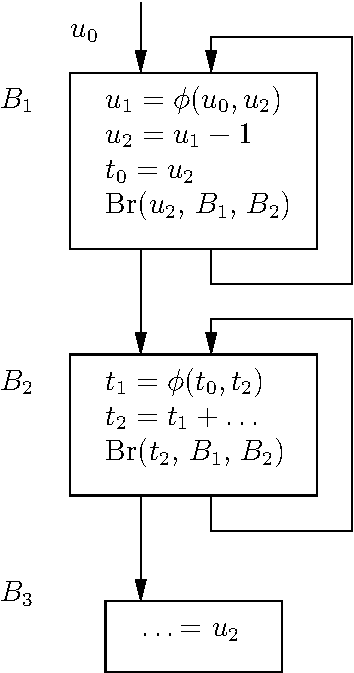
\includegraphics[scale=0.7]{cexple-impossible-1.pdf}\label{fig:alternative_ssa_destruction:ex_jump_impossible_a}
}
\hfill
\subfloat[Branch with decrement]{
    \hspace{2em}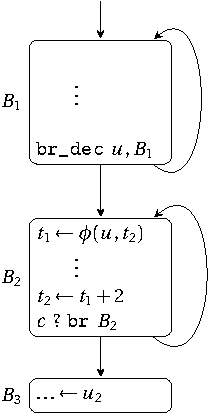
\includegraphics[scale=0.7]{cexple-impossible-2.pdf}\hspace{2em}\label{fig:alternative_ssa_destruction:ex_jump_impossible_b}
}
\hfill
\subfloat[C-SSA with additional edge splitting]{
    \hspace{1em}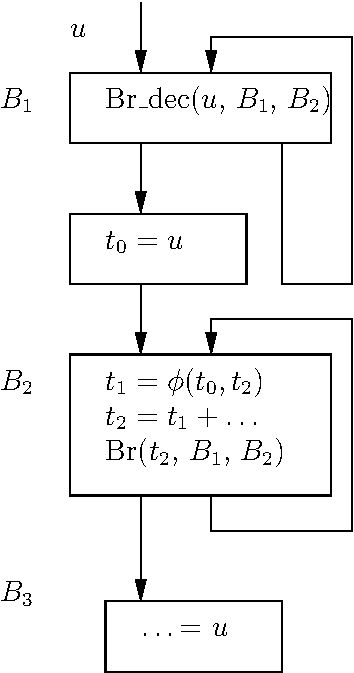
\includegraphics[scale=0.7]{cexple-impossible-3.pdf}\hspace{1em}\label{fig:alternative_ssa_destruction:ex_jump_impossible_c}
}
\caption{Copy insertion may not be sufficient. $\texttt{br\_dec}\ u,B_1$ decrements $u$, then branches to $B_1$ if $u\neq 0$.\label{fig:alternative_ssa_destruction:ex_jump_impossible}}
\end{figure}

There is another tricky case when a basic-block have twice the same predecessor block. This can result from consecutively applying copy-folding and control flow graph structural optimizations like dead code elimination or empty block elimination. This is the case for the example of Figure~\ref{fig:alternative_ssa_destruction:doublepreds} where copy-folding\index{copy-folding} would remove the copy $a_2\gets b$ in Block~$B_2$. If $B_2$ is eliminated, there is no way to implement the control dependence of the value to be assigned to $a_3$ other than through predicated code (see chapters~\ref{chapter:psi_ssa} and~\ref{chapter:vsdg}) or through the re-insertion of a basic-block between $B_1$ and $B_0$ by the split of one of the edges.

\begin{figure}[h]
\subfloat[Initial C-SSA code]{
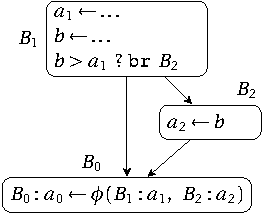
\includegraphics[scale=0.7]{doublepreds_a.pdf}
}\hfill
\subfloat[T-SSA code]{
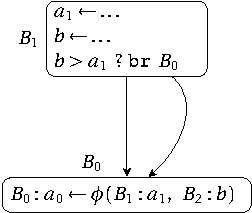
\includegraphics[scale=0.7]{doublepreds_b.pdf}
}\hfill
\subfloat[After $\phi$-isolation]{
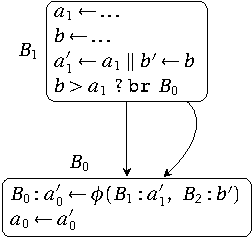
\includegraphics[scale=0.7]{doublepreds_c.pdf}
}\caption{\label{fig:alternative_ssa_destruction:doublepreds} Copy-folding followed by empty block elimination can lead to SSA code for which destruction is not possible through simple copy insertion}
\end{figure}


The last difficulty SSA destruction faces when performed at machine level is related to register constraints such as instruction set architecture (ISA)\index{instruction set architecture} or application binary interface (ABI)\index{application binary interface} constraints. For the sake of the discussion we differentiate two kinds of resource constraints that we will refer as \emph{operand pining}\index{pining} and \emph{live-range pining}. The live-range pining of a variable $v$ to resource $R$ will be represented $R_v$, just as if $v$ were a version of temporary $R$. An operand pining to a resource $R$ will be represented using the exponent $\pining{R}$ on the corresponding operand. 
Live-range pining expresses the fact that the \emph{entire} live-range of a variable must reside in a given resource (usually a dedicated register). An example of live-range pining are versions of the stack-pointer temporary that must be assigned back to register \SP. On the other hand the pining of an operation's operand to a given resource does not impose anything on the live-range of the corresponding variable. The scope of the constraint is restricted to the operation. Examples of operand pining are operand constraints such as \emph{2-address-mode} where two operands of one instruction must use the same resource; or where an operand must use a given register. This last case encapsulates ABI constraints. 
\begin{figure}[h]
\subfloat[Operand pining of an auto-increment]{
  \begin{minipage}{0.45\textwidth}
~\\
    \centerline{$p_2\pining{T}\gets p_1\pining{T}+1$}
~\\
  \end{minipage}
}
\hfill
\subfloat[Corresponding live-range pining]{
  \hspace{3em}\begin{minipage}{0.3\textwidth}
    $T_{p_1}\gets p_1$\\
    $T_{p_2}\gets T_{p_1}+1$\\
    $p_2\gets T_{p_2}$
  \end{minipage}
}
\\
\subfloat[Operand pining of a function call]{
  \begin{minipage}{0.4\textwidth}
~\\
    \centerline{$a\pining{R0}\gets f(b\pining{R0}, c\pining{R1})$}
~\\  \end{minipage}
}
\hfill
\subfloat[Corresponding live-range pining]{
  \hspace{3em}\begin{minipage}{0.3\textwidth}
    ${R0}_{b'}=b\ \parallel\ {R1}_{c'}=c$\\
    ${R0}_{a'}=f({R0}_{b'},{R1}_{c'})$\\
    $a={R0}_{a'}$
  \end{minipage}
}
\caption{\label{fig:alternative_ssa_destruction:pining}Operand pining and corresponding live-range pining}
\end{figure}

Note that looser constraints where the live-range or the operand can reside in more than one resource are not handled here. We assume this to always be the responsibility of register allocation.
We first simplify the problem by transforming any operand pining to a live-range pining as sketched in Figure~\ref{fig:alternative_ssa_destruction:pining}: parallel copies with new variables pinned to the corresponding resource are inserted just before (for \useop pining) and just after (for \defop pining) the operation.




{\bf Detection of strong interferences}
\label{par:alternative_ssa_destruction:strong}
The scheme we propose in this section to perform SSA destruction that deals with machine level constraints does not address compilation cost (in terms of speed and memory footprint). It is designed to be simple. It first inserts parallel copies to isolate \phifuns and operand pining. Then it checks for interferences that would persist. We will denote such interferences as strong, as they cannot be tackled through the simple insertion of temporary-to-temporary copies in the code. We consider that fixing strong interferences should be done on a case by case basis and restrict the discussion here on their detection.

As far as correctness is concerned, Algorithm~\ref{alg:alternative_ssa_destruction:sreedhar} splits the data flow between variables and \phinodes through the insertion of copies. For a given \phifun $a_0\gets \phi(a_1,\dots,a_n)$, this transformation is correct as long as the copies can be inserted close enough to the \phifun. It might not be the case if the insertion point (for a \useop) of copy $a'_i\gets a_i$ is not dominated by the definition point of $a_i$ (such as for argument $u$ of the \phifun $t_1\gets \phi(u,t_2)$ for the code of Figure~\ref{fig:alternative_ssa_destruction:ex_jump_impossible_b}); symmetrically, it will not be correct if the insertion point (for the \defop) of copy $a_0\gets a'_0$ does not dominate all the uses of $a_0$. Precisely this leads to inserting in Algorithm~\ref{alg:alternative_ssa_destruction:sreedhar} the following tests:
\begin{itemize}
\item line~\ref{line:sreedhar:1}: ``{\bf if} the definition of $a_i$ does not dominate $PC_i$ {\bf then} continue;''
\item line~\ref{line:sreedhar:2}: ``{\bf if} one use of $a_0$ is not dominated by $PC_0$ {\bf then} continue;''
\end{itemize}
For the discussion, we will denote as \emph{split operands} the newly created local variables to differentiate them to the ones concerned by the two previous cases (designed as \emph{non-split operands}).
% 
We suppose a similar process have been performed for operand pining to express them in terms of live-range pining with very short (when possible) live-ranges around the concerned operations. 

At this point, the code is still under SSA and the goal of the next step is to check that it is conventional: this will obviously be the case only if all the variables of a \phiweb can be coalesced together. But not only: the set of all variables pinned to a common resource must also be interference free. 
We say that $x$ and $y$ are \emph{pin-$\phi$-related} to one another if they are $\phi$-related or if they are pinned to a common resource. The transitive closure of this relation defines an equivalence relation that 
partitions the variables defined locally in the procedure into equivalence classes, the pin-$\phi$-webs.
Intuitively, the pin-$\phi$-equivalence class of a resource represents a set of resources ``connected'' via \phifuns and resource pining.
The computation of \phiwebs given by Algorithm~\ref{alg:ssadestruction:find-webs} can be generalized easily to compute pin-\phiwebs. The resulting pseudo-code is given by Algorithm~\ref{alg:alternative_ssa_destruction_algorithm:find-webs}. 

\begin{algorithm}[h]
  \Begin{
      \ForEach{$B$: basic block of the CFG}{
        insert an empty parallel copy at the beginning of $B$\;
        insert an empty parallel copy at the end of $B$\;
      }
      \ForEach{$B_0$: basic block of the CFG}{
        \ForEach{\phifun at the entry of $B_0$ of the form $a_0=\phi(B_1:a_1,\ldots,B_n:a_n)$}{
          \ForEach{$a_i$ (argument of the \phifun corresponding to $B_i$)}{
            \Let $PC_i$ be the parallel-copy at the end of $B_i$\;
            \nl\label{line:sreedhar:1} \BlankLine
            \Let $a'_i$ be a freshly created variable\;
            add copy $a'_i \gets a_i$ to $\mathrm{PC}_i$\;
            replace $a_i$ by $a'_i$ in the \phifun;
          }
          \Begin{
              \Let $PC_0$ be the parallel-copy at the beginning of $B_0$\;
              \nl\label{line:sreedhar:2} \BlankLine
              \Let $a'_0$ be a freshly created variable\;
              add copy $a_0 \gets a'_0$ to $\mathrm{PC}_0$\;
              replace $a_0$ by $a'_0$ in the \phifun\;
           }
          \tcc{all $a'_i$ can be coalesced and the \phifun removed}
        }
      }
    }
 \caption{\label{alg:alternative_ssa_destruction:sreedhar}Algorithm making non-conventional SSA form conventional by isolating \phinodes}
\end{algorithm}


Now, one need to check that each web is interference free. A web contains variables and resources. The notion of interferences between two variables is the one discussed in Section~\ref{sec:properties_and_flavors:ultimate_interference} for which we will propose an efficient implementation later in this chapter. A variable and a physical resource do not interfere while two distinct physical resources will interfere with one another.

If any interference have been discovered, it has to be fixed on a case by case basis. Note that some interferences such as the one depicted in Figure~\ref{fig:alternative_ssa_destruction:doublepreds} can be detected and handled initially (through edge splitting if possible) during the copy insertion phase.


\begin{algorithm}[h]
%% proc find_webs
%% // find the ssa web of each variable
\Begin{
\For{each resource $R$}{
  $\mathrm{web}(R)\gets \{R\}$\;
}
\For{each variable $v$}{
  $\mathrm{web}(v) \leftarrow \{v\}$\;
  \If{$v$ pinned to a resource $R$}{
    union$(\mathrm{web}(R),\mathrm{web}(v))$
 }
}
\For{each instruction of the form $a_{\mathrm{dest}} = \phi(a_1,\ldots,a_n)$}{
  \For{each source operand $a_i$ in instruction}{
     union$(\mathrm{web}(a_{\mathrm{dest}}),\mathrm{web}(a_i))$
  }
}
}
\caption{\label{alg:alternative_ssa_destruction_algorithm:find-webs}The pin-\phiwebs discovery algorithm, based on the union-find pattern}
\end{algorithm}
